% Policy architecture figures for "Learning Inventory Control Policies with Evolution Strategies".
% Visual style adapted from Izaak Neutelings (Sept 2021), neural-network-zoo TikZ
% (https://www.asimovinstitute.org/neural-network-zoo/), as used in the prior version of the paper.
%
% This standalone document compiles to a multi-page PDF; include individual pages in the
% manuscript with 
\includegraphics[page=N]{figures/policy_architecture.pdf}:
%   page 1: the policy pipeline / contract  (state -> normalize -> backbone -> decoder -> valid action)
%   page 2: the NN backbone (state s_1..s_L -> hidden layer H -> latent outputs u)
%   page 3: the decoder heads (direct / ordinal / categorical / soft-tree leaves -> integer order)
%
% Build:  pdflatex policy_architecture.tex   (or tectonic policy_architecture.tex)
\documentclass[border=3pt,tikz]{standalone}
\usepackage{amsmath}
\DeclareMathOperator*{\argmax}{arg\,max}
\usepackage{tikz}
\usepackage{listofitems}
\usetikzlibrary{arrows.meta,positioning,fit,backgrounds}
\usepackage[outline]{contour}
\contourlength{1.4pt}

\tikzset{>=latex}
\usepackage{xcolor}
\colorlet{myred}{red!80!black}
\colorlet{myblue}{blue!80!black}
\colorlet{mygreen}{green!60!black}
\colorlet{myorange}{orange!70!red!60!black}
\colorlet{mydarkred}{red!30!black}
\colorlet{mydarkblue}{blue!40!black}
\colorlet{mydarkgreen}{green!30!black}
\tikzstyle{node}=[thick,circle,draw=myblue,minimum size=22,inner sep=0.5,outer sep=0.6]
\tikzstyle{node in}=[node,green!20!black,draw=mygreen!30!black,fill=mygreen!25]
\tikzstyle{node hidden}=[node,blue!20!black,draw=myblue!30!black,fill=myblue!20]
\tikzstyle{node out}=[node,red!20!black,draw=myred!30!black,fill=myred!20]
\tikzstyle{connect}=[thick,mydarkblue]
\tikzstyle{connect arrow}=[-{Latex[length=4,width=3.5]},thick,mydarkblue,shorten <=0.5,shorten >=1]
% box styles for the pipeline figure
\tikzstyle{stage}=[rounded corners=3pt,thick,minimum height=14mm,align=center,inner sep=6pt]
\tikzstyle{stage in}=[stage,draw=mygreen!50!black,fill=mygreen!12]
\tikzstyle{stage mid}=[stage,draw=myblue!50!black,fill=myblue!10]
\tikzstyle{stage dec}=[stage,draw=myorange!60!black,fill=myorange!12]
\tikzstyle{stage out}=[stage,draw=myred!50!black,fill=myred!15]
\tikzstyle{flow}=[-{Latex[length=5,width=4]},thick,mydarkblue]

\begin{document}


% =====================================================================
% PAGE 1 -- POLICY PIPELINE / CONTRACT: input = state  ->  valid action
% Everything between the input state and the output action is the policy.
% =====================================================================
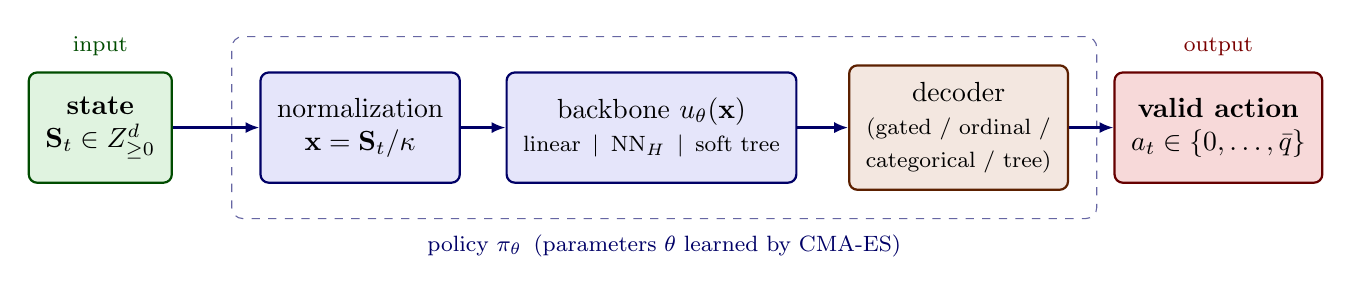
\begin{tikzpicture}[x=1cm,y=1cm]
  \node[stage in]  (s)   at (0,0)  {\textbf{state}\\$\mathbf{S}_t\in\mathbb{Z}_{\ge0}^{d}$};
  \node[stage mid] (nrm) at (3.3,0){normalization\\$\mathbf{x}=\mathbf{S}_t/\kappa$};
  \node[stage mid] (bb)  at (7.0,0){backbone $u_\theta(\mathbf{x})$\\\footnotesize linear \,$\mid$\, NN$_H$ \,$\mid$\, soft tree};
  \node[stage dec] (dec) at (10.9,0){decoder\\\footnotesize (gated / ordinal /\\\footnotesize categorical / tree)};
  \node[stage out] (a)   at (14.2,0){\textbf{valid action}\\$a_t\in\{0,\dots,\bar q\}$};

  \draw[flow] (s)   -- (nrm);
  \draw[flow] (nrm) -- (bb);
  \draw[flow] (bb)  -- (dec);
  \draw[flow] (dec) -- (a);

  % brace: everything between input and output is the (learned) policy
  \begin{scope}[on background layer]
    \node[draw=mydarkblue!60,dashed,rounded corners=4pt,inner sep=10pt,
          fit=(nrm)(bb)(dec)] (pol) {};
  \end{scope}
  \node[mydarkblue,below=2pt of pol.south] {\footnotesize policy $\pi_\theta$ \,(parameters $\theta$ learned by CMA-ES)};
  \node[mygreen!50!black,above=2pt of s.north]  {\footnotesize input};
  \node[myred!60!black,above=2pt of a.north]    {\footnotesize output};
\end{tikzpicture}


% =====================================================================
% PAGE 2 -- NN BACKBONE: state vector -> hidden layer -> latent outputs
% (adapted from the prior version's neural-network figure)
% =====================================================================
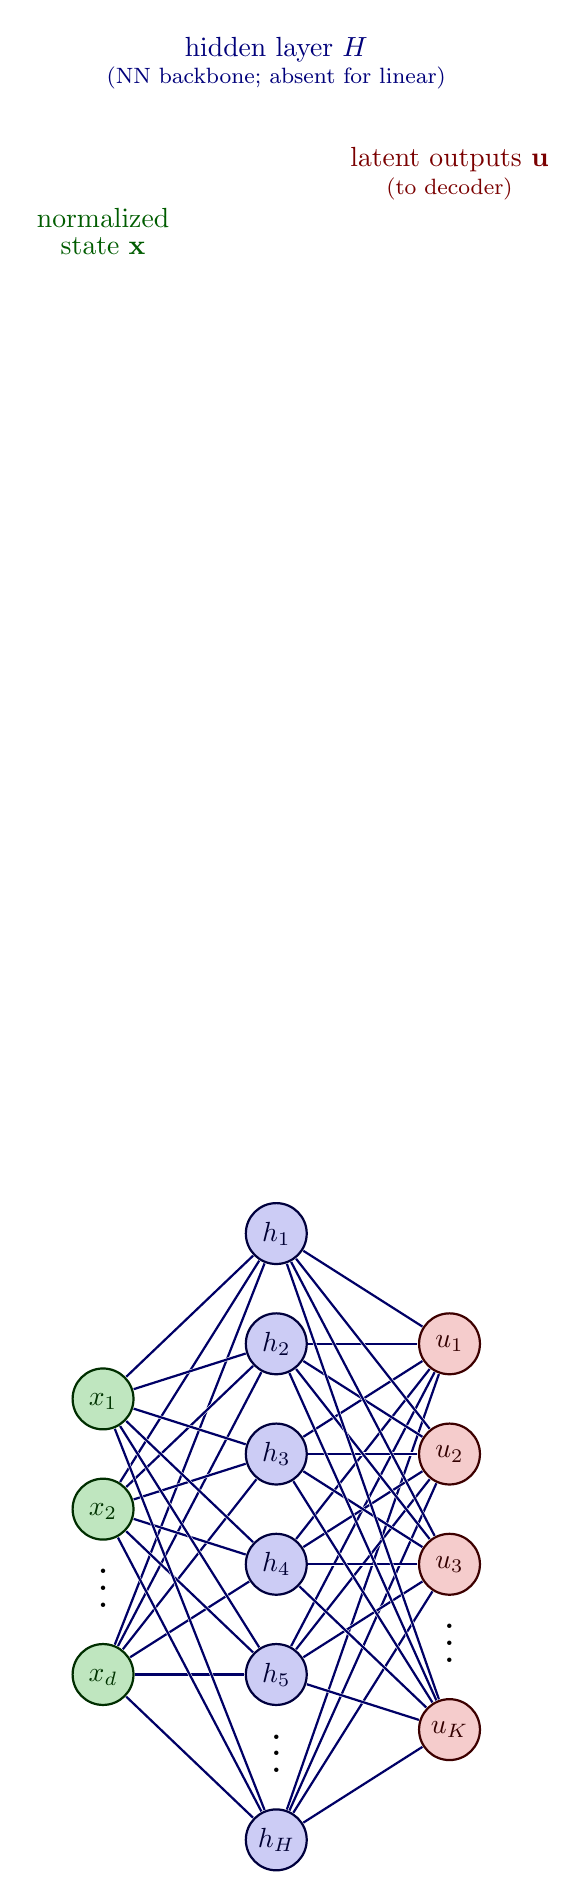
\begin{tikzpicture}[x=2.2cm,y=1.4cm]
  \readlist\Nnod{3,6,4}        % nodes per layer: d (=L), H, K (latent outputs)
  \readlist\Nstr{d,H,K}        % size symbols per layer
  \readlist\Cstr{\strut x,h,u} % coefficient symbol per layer
  \def\yshift{0.5}

  \foreachitem \N \in \Nnod{
    \def\lay{\Ncnt}
    \pgfmathsetmacro\prev{int(\Ncnt-1)}
    \foreach \i [evaluate={\c=int(\i==\N); \y=\N/2-\i-\c*\yshift;
                 \index=(\i<\N?int(\i):"\Nstr[\lay]");
                 \x=\lay; }] in {1,...,\N}{
      \ifnum\lay=1
        \node[node in]     (N\lay-\i) at (\x,\y) {$\Cstr[\lay]_{\index}$};
      \else\ifnum\lay=\Nnodlen
        \node[node out]    (N\lay-\i) at (\x,\y) {$\Cstr[\lay]_{\index}$};
      \else
        \node[node hidden] (N\lay-\i) at (\x,\y) {$\Cstr[\lay]_{\index}$};
      \fi\fi
      \ifnum\lay>1
        \foreach \j in {1,...,\Nnod[\prev]}{
          \draw[connect,white,line width=1.2] (N\prev-\j) -- (N\lay-\i);
          \draw[connect] (N\prev-\j) -- (N\lay-\i);
        }
      \fi
    }
    \path (N\lay-\N) --++ (0,1+\yshift) node[midway,scale=1.5] {$\vdots$};
  }
  \node[above=10,align=center,mygreen!60!black] at (N1-1.90) {normalized\\[-0.2em]state $\mathbf{x}$};
  \node[above=10,align=center,myblue!60!black]  at (N2-1.90) {hidden layer $H$\\[-0.2em]\footnotesize (NN backbone; absent for linear)};
  \node[above=10,align=center,myred!60!black]   at (N\Nnodlen-1.90) {latent outputs $\mathbf{u}$\\[-0.2em]\footnotesize (to decoder)};
\end{tikzpicture}


% =====================================================================
% PAGE 3 -- DECODER HEADS: latent outputs u -> integer order a
% Each head is part of the policy; all map to a valid (non-negative integer) action.
% =====================================================================
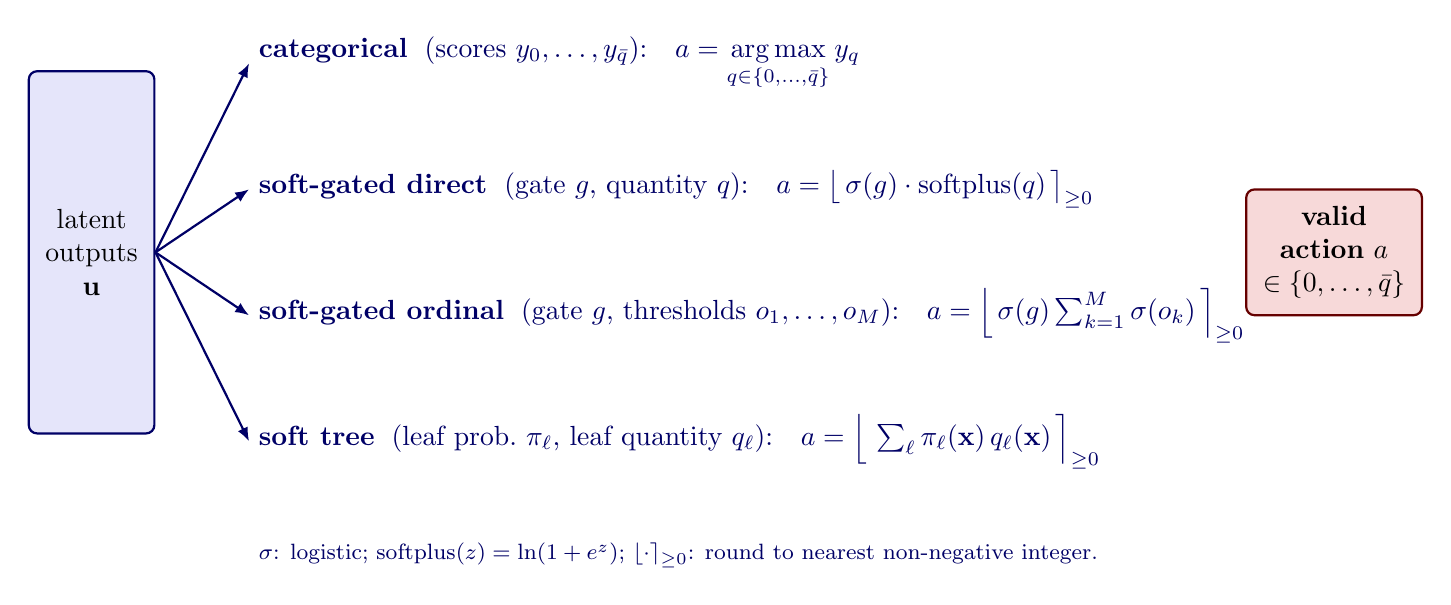
\begin{tikzpicture}[x=1cm,y=1cm,every node/.style={align=left}]
  \def\rowsep{1.6}
  \node[stage mid,minimum height=46mm] (u) at (0,-2.4) {latent\\outputs\\$\mathbf{u}$};

  % categorical (the classical argmax score head)
  \node[anchor=west,mydarkblue] (d0) at (2,0)
    {\textbf{categorical} \;(scores $y_0,\dots,y_{\bar q}$):\quad
     $a=\displaystyle\argmax_{q\in\{0,\dots,\bar q\}} y_q$};
  % soft-gated direct
  \node[anchor=west,mydarkblue] (d1) at (2,-\rowsep)
    {\textbf{soft-gated direct} \;(gate $g$, quantity $q$):\quad
     $a=\big\lfloor\, \sigma(g)\cdot\mathrm{softplus}(q)\,\big\rceil_{\ge0}$};
  % soft-gated ordinal
  \node[anchor=west,mydarkblue] (d2) at (2,-2*\rowsep)
    {\textbf{soft-gated ordinal} \;(gate $g$, thresholds $o_1,\dots,o_M$):\quad
     $a=\Big\lfloor\, \sigma(g)\sum_{k=1}^{M}\sigma(o_k)\,\Big\rceil_{\ge0}$};
  % soft tree
  \node[anchor=west,mydarkblue] (d3) at (2,-3*\rowsep)
    {\textbf{soft tree} \;(leaf prob.\ $\pi_\ell$, leaf quantity $q_\ell$):\quad
     $a=\Big\lfloor\, \sum_{\ell}\pi_\ell(\mathbf{x})\,q_\ell(\mathbf{x})\,\Big\rceil_{\ge0}$};

  \foreach \d in {d0,d1,d2,d3}{ \draw[flow] (u.east) -- (\d.west); }

  \node[stage out,right=18mm of d1.east,yshift=-8mm] (a) {\textbf{valid}\\\textbf{action} $a$\\$\in\{0,\dots,\bar q\}$};
  \node[mydarkblue,below=7mm of d3.south west,anchor=north west]
    {\footnotesize $\sigma$: logistic; $\mathrm{softplus}(z)=\ln(1+e^z)$; $\lfloor\cdot\rceil_{\ge0}$: round to nearest non-negative integer.};
\end{tikzpicture}


\end{document}
